\documentclass[./../../paper.tex]{subfiles}
\graphicspath{{\subfix{./../../figures/}}}

\begin{document}



The architecture of the prediction model is shown in \autoref{fig:lstm_architecture}. The model architecture is inspired by \citeauthor{hsieh_DiCE4ELInterpretingProcess_2021}. However, we do not separate the input into dynamic and static features.

One input consists of a 2-dimensional event tensor containing integers. The second input is a 3-dimensional tensor containing the remaining feature attributes. The first dimension in each layer represents the variable batch size, and \emph{None} acts as a placeholder.

The next layer is primarily concerned with preparing the full vector representation. We encode each activity in the sequence into a vector space. We chose a dense-vector representation instead of a one-hot representation. We also create positional embeddings. Then we concatenate the activity embedding, positional embedding and the event attribute representation to a final vector representation for the event that occurred.

Afterwards, we pass the tensor through a \gls{LSTM} module. We use the output of the last step to predict the outcome of a sequence using a fully connected neural network layer with a sigmoid activation as this is a binary classification task. 

\begin{figure}[htbp]
    \centering
    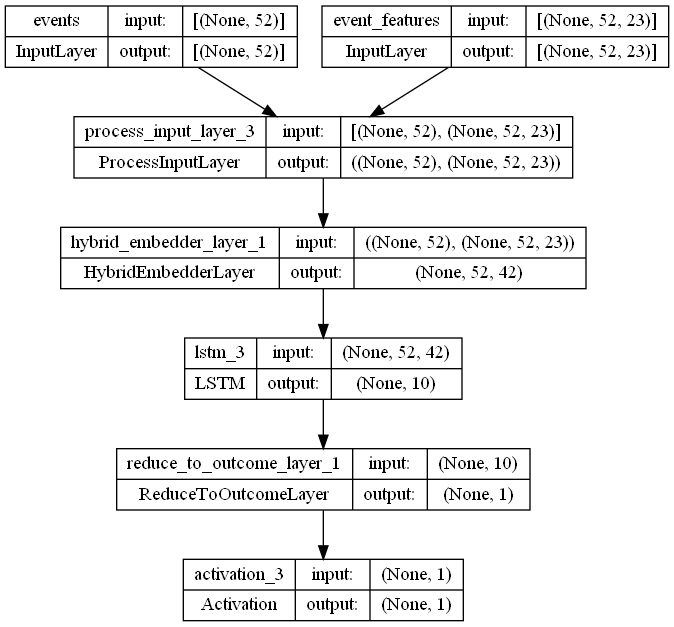
\includegraphics[width=0.8\textwidth]{figures/predictor50lstm.png}
    \caption{The different components of the LSTM architecture. Each element contains information about the input and output of a layer. None is a placeholder for the batch size.}
    \label{fig:lstm_architecture}
\end{figure}

% \subsection{Transformer Model}
% Transformer models are modern sequential models within \gls{DL}. They have a multitude of advantages over sequential models such as \glspl{RNN} or \glspl{LSTM}\autocite{vaswani_AttentionAllYou_2017}. First, they do not need to be computed sequentially. Hence, it is possible to parallelise the training and inference substantially using GPUs. Second, they can take the full sequence as an input using the attention mechanism. This mechanism also allows for inspecting which inputs have had a significant role in producing the prediction. However, transformer models are more complicated to implement. The overall setup is shown in \autoref{fig:transformer}\autocite{vaswani_AttentionAllYou_2017}.

% \begin{figure}[htb]
%     \centering
%     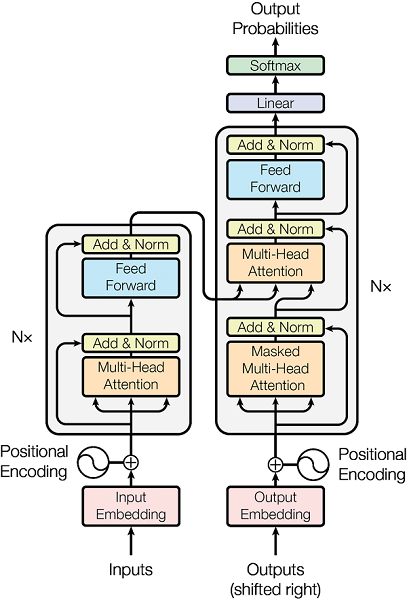
\includegraphics[width=0.5\textwidth]{figures/transformer.png}
%     \caption{A schematic representation of a Transformer model.}
%     \label{fig:transformer}
% \end{figure}

% The transformer model is an Encoder-Decoder model. The encoder takes in the input sequence as a whole and generates a vector which encodes the information. The decoder uses the encoding to produce the resulting sequence. The encoder module uses two important concepts. First, to preserve the input's temporal information, we encode each sequential input's position as an additional input vector. We choose to encode every position by jointly learning positional embeddings. The second component is multi head-self-attention. According to \citeauthor{vaswani_AttentionAllYou_2017}, we can describe attention as a function which maps a query and a set of key-value pairs to an output. More specifically, self-attention allows us to relate every input element in the sequence to be related to any other sequence in the input. The output is a weighted sum of the values. It is possible to stack multiple self-attention modules. This procedure is called multi-head-attention. \autoref{fig:selfattention} shows how to compute self-attention according to \autoref{eq:selfattention}\autocite{vaswani_AttentionAllYou_2017}. 


% \begin{figure}[htb]
%     \centering
%     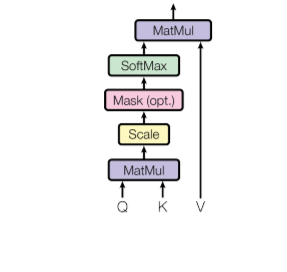
\includegraphics[width=0.5\textwidth]{figures/selfattention.png}
%     \caption{The computational graph of self-attention. $Q, K \text{ and } V$ are all the same input sequence. $Q$ stands for query, $K$ for key and $V$ for value.}
%     \label{fig:selfattention}
% \end{figure}


% \begin{align}
%     \label{eq:selfattention}
%     Attention(Q, K, V) &= softmax(\frac{QK^T}{\sqrt{d_k}})V 
% \end{align}

% $Q, K, V$ are all the same input sequence. $d_k$ refers to the dimension of an input vector. Note that $T$ is the transpose operation of matrix computations and does not relate to the time step of the final sequence element. 




\end{document}